\documentclass[a4paper, 12pt]{article}

%%% Работа с русским языком
\usepackage{cmap}					% поиск в PDF
\usepackage{mathtext} 				% русские буквы в формулах
\usepackage[T2A]{fontenc}			% кодировка
\usepackage[utf8]{inputenc}			% кодировка исходного текста
\usepackage[russian]{babel}	% локализация и переносы

%%% Дополнительная работа с математикой
\usepackage{amsmath,amsfonts,amssymb,amsthm,mathtools} % AMS
\usepackage{icomma} % "Умная" запятая: $0,2$ --- число, $0, 2$ --- перечисление

%% Номера формул
%\mathtoolsset{showonlyrefs=true} % Показывать номера только у тех формул, на которые есть \eqref{} в тексте.

%% Шрифты
\usepackage{euscript}	 % Шрифт Евклид
\usepackage{mathrsfs} % Красивый матшрифт

%% Поля
\usepackage[left=2cm,right=2cm,top=2cm,bottom=2cm,bindingoffset=0cm]{geometry}

%% Русские списки
\usepackage{enumitem}
\makeatletter
\AddEnumerateCounter{\asbuk}{\russian@alph}{щ}
\makeatother

%%% Работа с картинками
\usepackage{graphicx}  % Для вставки рисунков
\graphicspath{{images/}{images2/}}  % папки с картинками
\setlength\fboxsep{3pt} % Отступ рамки \fbox{} от рисунка
\setlength\fboxrule{1pt} % Толщина линий рамки \fbox{}
\usepackage{wrapfig} % Обтекание рисунков и таблиц текстом

%%% Работа с таблицами
\usepackage{array,tabularx,tabulary,booktabs} % Дополнительная работа с таблицами
\usepackage{longtable}  % Длинные таблицы
\usepackage{multirow} % Слияние строк в таблице

%% Красная строка
\setlength{\parindent}{2em}

%% Интервалы
\linespread{1}
\usepackage{multirow}

%% TikZ
\usepackage{tikz}
\usetikzlibrary{graphs,graphs.standard}

%% Верхний колонтитул
\usepackage{fancyhdr}
\pagestyle{fancy}

%% Перенос знаков в формулах (по Львовскому)
\newcommand*{\hm}[1]{#1\nobreak\discretionary{}
	{\hbox{$\mathsurround=0pt #1$}}{}}

%% Мои дополнения
\usepackage{float} %Добавляет возможность работы с командой [H] которая улучшает расположение на странице
\usepackage{gensymb} %Красивые градусы
\usepackage{graphicx}               % Импорт изображений
\usepackage{caption} % Пакет для подписей к рисункам, в частности, для работы caption*
\usepackage{indentfirst}


\begin{document}

\newcommand{\HRule}{\rule{\linewidth}{0.7mm}} % Defines a new command for the horizontal lines, change thickness here
	
	\begin{center}
		\large\textbf{Московский Физико-Технический Институт}\\ % Name of your university/college
		\large\textbf{(государственный университет)}
	
		\vfill
		
		\Large Лабораторная работа по курсу общей физики № 4.5.3\\[0.5cm] % Preambule of your document title
		
		
		\HRule
		\\[0.4cm]
		{ \huge \bfseries Сканирующий интерферометр}% Title of your document
		\\[0.4cm] 
		\HRule
		\\[0.5cm]
		
		\ \\
	\textbf{\large Автор:} \\	
	\large Лепарский Роман Б01-003\\ % Your name and something more, your group num for example
		\vfill
		\hspace*{-0.8 cm}
\includegraphics[width=100 pt]{frkt_logo}\\ % logo of your  company/university/college
		\large Долгопрудный, 2022 % location and year
	\end{center}

\newpage
\setcounter{page}{2}
\fancyfoot[c]{\thepage}
\fancyhead[L] {Работа № 4.5.3} % some information in page header
\fancyhead[R]{}
\section{Аннотация}
\textbf{Цель работы}: исследовать интерференцию рассеянного света, прошедшего кристалл; наблюдать изменение характера поляризации света при наложении на кристалл электрического поля.

\textbf{Приборы и материалы}: гелий-неоновый лазер, поляризатор, кристалл ниобата лития, матовая пластина, экран, источник высоковольтного переменного и постоянного напряжения, фотодиод, осцилограф, линейка.


\section{Теоретические сведения}

Эффект Поккельса -- изменение показателя преломления света в кристалле под действием электрического поля.
Рассмотрим кристалл ниобата лития $\text{LiNbO}_3$ с цетрольноосевой симметрией вдоль оси $Z$. Для световой волны с $\mathbf{E}$ перпендикулярно $Z$ показатель преломления будет $n_o$, а для волны с $\mathbf{E}$ вдоль $Z$ -- $n_e$. В случае, когда луч света идёт под углом $\theta$ к оси, есть два значение показателя преломления $n_1$ и $n_2$: $n_1 = n_o$ для волны с $\mathbf{E}$ перпендикулярным плоскости $(\mathbf{k},\mathbf{Z})$ (обыкновенная волна) и $n_2$ для волны с $\mathbf{E}$ в этой плоскости (необыкновенная волна). В последнем случае
\begin{equation}
\dfrac{1}{n_2^2}=\dfrac{\cos^2 \theta}{n_0^2}+\dfrac{\sin^2 \theta}{n_e^2}.
\end{equation}

\begin{figure}[H]
	\begin{center}
		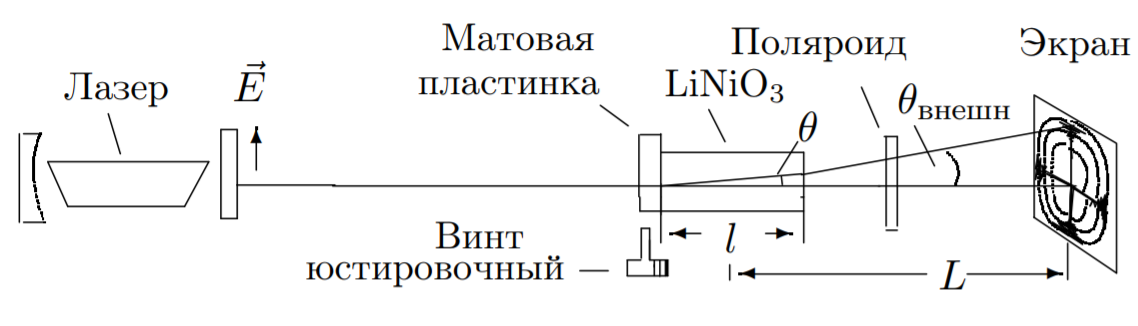
\includegraphics[scale = 0.5]{1.png}
	\end{center}
	\caption{Схема для наблюдения интерференционной картины.}
\end{figure}
%\begin{figure}[h!]
%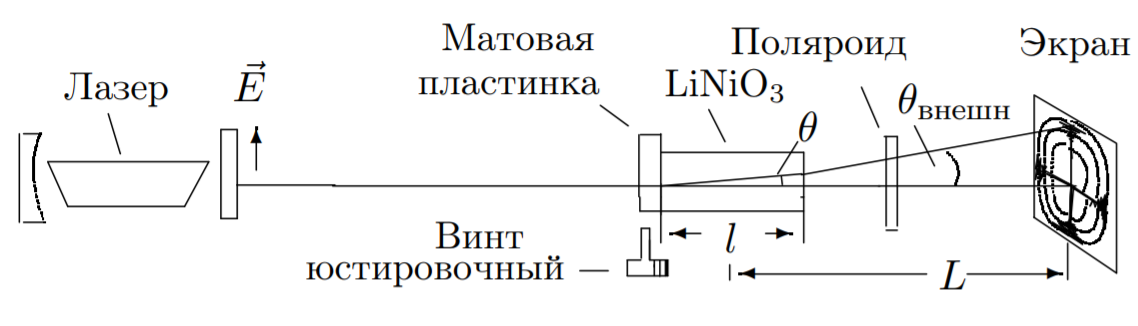
\includegraphics[scale=0.5]{1.png}
%\centering
%\caption{Схема для наблюдения интерфереционной картины}
%\end{figure}
Если перед кристаллом, помещённым между поляроидами, расположить линзу или матовую пластинку, то на экране за поляроидом мы увидим тёмные концентрические окружности -- рещультат интерфернции обыкновенной и необыкновенной волн. При повороте выходного поляроида на $90^\circ$ картина меняется с позитива на негатив (на месте светлых пятен тёмные и наоборот). В случаи, когда разрешённое направление анализатора перпендикулярно поляризации лазерного излучения, радиус тёмного кольца с номером $m$ равен
\begin{equation}
r_m^2 = \dfrac{\lambda}{l} \dfrac{(n_oL)^2}{n_0 - n_e}m,
\end{equation}
где $L$ -- расстояние от центра кристалла до экрана, $l$ -- длина кристалла.\\
Теперь поместим кристалл в постоянное электрическое поле $E_{\text{эл}}$, направленное вдоль оси $X$, перпендикулярной $Z$. Показатель преломления для луча, распространяющего вдоль $Z$, всегда $n_o$. В плоскости $(X,Y)$ возникают два главных направления под углами $45^\circ$ к $X$ и $Y$ с показателями преломления $n_0 - \Delta n$ и $n_o + \Delta n$ (быстрая и медленная ось), причём $\Delta n = A E_{\text{эл}}$. Для поляризованного вертикально света и анализатора, пропускающего горизонтальную поляризацию, на выходе интенсивность на выходе будет иметь вид
\begin{equation}
I_{\text{вых}} = I_0 \sin^2 \left(\dfrac{\pi}{2} \dfrac{U}{U_{\lambda/2}} \right),
\end{equation}
где $U_{\lambda/2} = \frac{\lambda}{4A}\frac{d}{l}$ -- \textit{полуволновое напряжение}, $d$ -- поперечный размер кристалла.  При напряжении $U = E_{\text{эл}}d$ равном полуволновому сдвиг фаз между двумя волнами равен $\pi$, а интенсивность света на выходе максимальна. 


\begin{figure}[H]
	\begin{center}
		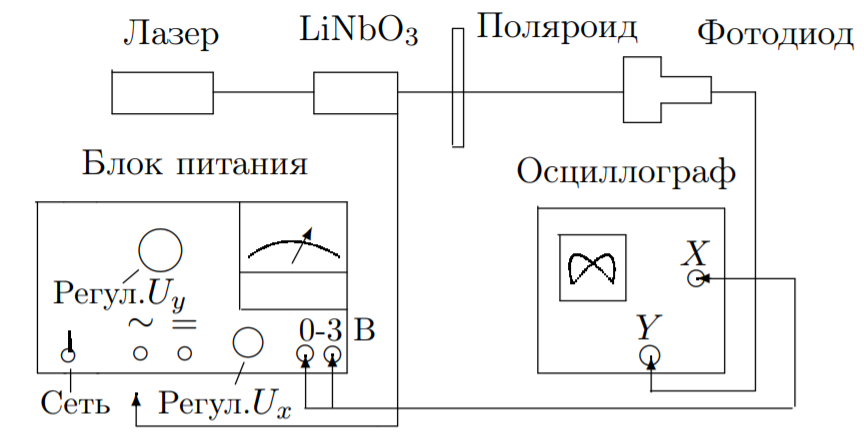
\includegraphics[scale = 0.5]{2.png}
	\end{center}
	\caption{Схема установки.}
\end{figure}
На Рис. 2 представлена схема всей установки (оптическая часть изорбажена на Рис. 1). Свет лазера, проходя через сквозь пластину, рассеивается и падает на двоякопреломляющий кристалл. На экране за поляроидом видна интерференционная картина. Убрав рассеивающую пластину и подавая на кристалл постоянное напряжение, можно величиной напряжения влиять на поляризацию луча, вышедшего из кристалла. Заменив экран фотодиодом и подав на кристалл переменное напряжение, можно исследовать поляризацию с помощью осциллографа.

	\section{Обработка результатов}
	После юстировки системы измерим расстояние от центра кристалла до экрана $L = 73,7\pm0,5$ см, длина кристалла $l = 26$ мм, показатель преломления $n_0 = 2,29$, и длина волны лазера $630$ нм.
	
	Запишем радиусы темных колец
	\begin{table}[H]
		\centering
		\begin{tabular}{|l|l|l|l|l|l|l|l|l|l|}
			\hline
			$m$       & 1    & 2    & 3    & 4    & 5    & 6    & 7    & 8    & 9    \\ \hline
			$r_m$, мм & 27,0 & 38,0 & 47,5 & 54,5 & 61,0 & 67,5 & 72,5 & 77,5 & 82,0 \\ \hline
		\end{tabular}
	\end{table}

	Построим график $r^2 = f(m)$
	\begin{figure}[H]
		\begin{center}
			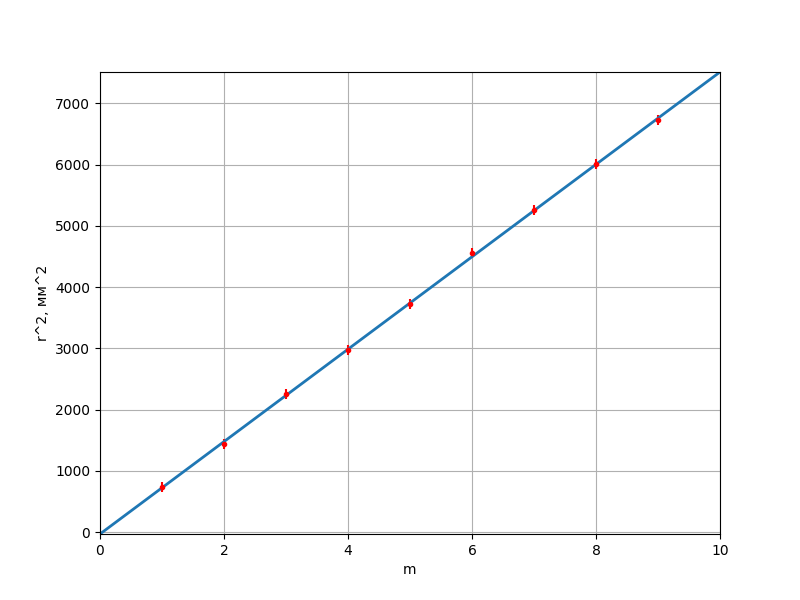
\includegraphics[scale = 0.7]{3}
		\end{center}
	\end{figure}
	Коэффициент наклона $\alpha = 754\pm3$ мм$^2$. Рассчитаем разность показателей преломления по формуле
	\[
		n_0 - n_e = \frac{\lambda}{l}\frac{(n_0L)^2}{\alpha} = 0,0912
	\]
	\[
	\sigma_n = \frac{\lambda}{l}\frac{(n_0L)^2}{\alpha^2}\cdot\sigma_\alpha = 0,0003
	\]
	Табличное значение $n_0 - n_e = 0,09$ совпадает с рассчитанным.
	
	Теперь подключим к кристаллу блок питания с постоянным напряжением. Максимальная интенсивность света при скрещенных поляроидах наблюдается при $U_{max} = 480\pm30$ В, минимальная интенсивность: $U_{min} = 960\pm30$ В. Таким образом, полуволновое напряжение $U_{\lambda/2} = 480 \pm 30$ В. Для параллельных поляроидов значения такие же. Погрешность обусловлена тем, что невозможно определить точный минимум и максимум интенсивности.
	
	На следующем этапе поставим вместо экрана фотодиод и подадим на кристалл переменное напряжение. По фигурам Лиссажу определим напряжения:
	\[
		U_{\lambda/2} = 420 \pm 15 \text{ В}
	\]
	\[
		U_{\lambda} = 870 \pm 15\text{ В}
	\]
	\[
		U_{3\lambda/2} = 1350 \pm 15\text{ В}
	\]
	
	При изменении разрешенного направления анализатора на перпендикулярное фигура Лиссажу отражается относительно горизонтали.
	
	\section{Вывод}
	В данной работе мы исследовали интерференцию света, прошедшего через кристалл. А так же наблюдали изменение характера поляризации света при наложении на кристалл напряжения.









	

	
	
	
	
	
	
	
	
	
	
	
	
	
	
	
	
	

\end{document}